\documentclass[runningheads]{llncs}

\usepackage[T1]{fontenc}
\usepackage{graphicx}
% \renewcommand\UrlFont{\color{blue}\rmfamily}
\usepackage{hyperref}
\usepackage{color}
\usepackage{setspace}
\usepackage{verbatim}
\usepackage{multicol}
\usepackage{array}
\newcommand{\PreserveBackslash}[1]{\let\temp=\\#1\let\\=\temp}
\newcolumntype{C}[1]{>{\PreserveBackslash\centering}p{#1}}
\newcolumntype{R}[1]{>{\PreserveBackslash\raggedleft}p{#1}}
\newcolumntype{L}[1]{>{\PreserveBackslash\raggedright}p{#1}}
\setlength{\tabcolsep}{3pt}

\renewcommand{\floatpagefraction}{0.9}
\renewcommand{\textfloatsep}{2.0ex}
\renewcommand{\dbltextfloatsep}{2.0ex}

\newenvironment{packed_itemize}{
\vspace*{-0.5em}
\begin{itemize}
\setlength{\partopsep}{0pt}
\setlength{\itemsep}{1pt}
\setlength{\parskip}{0pt}
\setlength{\parsep}{0pt}
}{\end{itemize}}

\begin{document}

\title{An Empirical Assessment of Progress in \\ Automated Theorem Proving}
\titlerunning{Progress in ATP}

\author{
Geoff Sutcliffe\inst{1}\orcidID{0000-0001-9120-3927}
\and
Christian Suttner\inst{2}
\and \\
Lars Kotthoff\inst{3}\orcidID{0000-0003-4635-6873}
\and \\
C. Raymond Perrault\inst{4}\orcidID{0009-0001-1178-343X}
\and \\
Zain~Khalid\inst{1}\orcidID{0009-0001-2063-6933}
}
\authorrunning{G. Sutcliffe, et al.}
\institute{University of Miami, USA,
\email{geoff@cs.miami.edu},
\email{zsk17@miami.edu}
\and
Deceased
\and 
University of Wyoming, USA,
\email{larsko@uwyo.edu}
\and 
SRI International, USA,
\email{ray.perrault@sri.com}
}

\maketitle
%--------------------------------------------------------------------------------------------------
\begin{abstract}
The TPTP World is a well established infrastructure that supports research, development, and 
deployment of Automated Theorem Proving (ATP) systems.
This work uses data in the TPTP World to assess progress in ATP from 2015 to 2023.
% The analyses clearly show progress, but an apparent slowing of progress compared to the
% prior five years.

\keywords{Automated Theorem Proving \and Empirical Evaluation \and Progress}
\end{abstract}
%--------------------------------------------------------------------------------------------------
\section{Introduction}
\label{Introduction}

The TPTP World \cite{Sut17} (\href{https://www.tptp.org}{\tt www.tptp.org}) is a well established 
infrastructure that supports research, development, and deployment of Automated Theorem Proving 
(ATP) systems.
The TPTP World includes the TPTP problem library,
% \cite{Sut09}, 
the TSTP solution library,
% \cite{Sut10}, 
standards for writing ATP problems and reporting ATP solutions,
% \cite{SS+06,Sut08-KEAPPA}, 
tools and services for processing ATP problems and solutions,
% \cite{Sut10}, 
and it supports the CADE ATP System Competition (CASC).
% \cite{Sut16}.
% Various parts of the TPTP World have been deployed in a range of applications,
% in both academia and industry.
This work uses data in the TPTP World to assess progress in ATP from 2015 to 2023.

Any meaningful assessment of progress in ATP must refer to the ability of ATP systems to solve 
problems.
As the systems improve over time, the problems that they must solve also change to meet 
the demands of applications (with a fixed set of problems the systems can simply be finely 
tuned to the set, with inevitable asymptotic progress towards solving all the problems 
\cite{OB+22}).
The TPTP problem library provides an evolving set of ATP problems that reflect the needs of 
ATP users, and is an appropriate basis for assessing the changing ability of ATP systems.
Alongside the TPTP problem library, the TSTP solution library provides data about ATP systems' 
abilities to solve the problems in the TPTP problem library.
This paper examines progress in ATP, based on the data from TPTP v6.3.0 released on 
28th November 2015 to TPTP v8.2.0 released on 13th June 2023.
It is important to differentiate between evaluations at instances in time, such as provided by
competitions, and evaluations over time.
At instances of time the test problems used for evaluation, the systems being evaluated, and
the hardware/software platform used, are static, e.g., as done in \cite{CSW15}.
That provides a clean basis for a detailed comparison between systems.
In contrast, evaluation over time is complicated by changing test problems, changing systems,
and changing hardware/software.
This dynamic evaluation environment requires additional control to provide meaningful results.
The analyses done in this work do not explicitly factor in the resources needed to find solutions, 
e.g., hardware, time limits, etc; Section~\ref{ResourceLimits} explains why this makes sense in 
the ATP context.

\paragraph{Related work:}
The use of system performance data to evaluate a field of endeavour is common.
In the realm of logic-based systems, examples include
the various competitions \cite{BB+19} for logic-based systems (e.g., CASC \cite{Sut16}, the SAT 
Competition \cite{JL+12}, SMT-COMP \cite{BdS05}, the ASP Competition \cite{CI+12}),
longitudinal surveys of competitions \cite{SS06-SoCASC,CSW15},
the Technical Performance chapter of Stanford University's AI Index Annual Report \cite{MF+23},
the use of Shapley values to evaluate algorithmic improvements in SAT solving \cite{FK+16,KF+19},
comparison of algorithmic and hardware advances (in SAT solving) \cite{FHS20},
and
other more specialized benchmarking, e.g., \cite{ZHP22}.
A general examination of the requirements for such benchmarking is provided by \cite{BLW19}.
An ontology of artificial intelligence benchmarks is described in \cite{BB+22-SD}.
\cite{OB+22} provides an insightful analysis of the global dynamics of using benchmark sets in
computer vision and natural language processing, and the takeaway messages are broadly applicable,
including to benchmark sets for logic-based systems.
In all cases the common measures for evaluation are (i)~the ability of systems to solve problems, 
and (ii)~the resources required by the systems to solve the problems.
In order for results to be relevant, test problems must be representative of the problems
the systems will face in applications, and the resource measurements must be appropriate for 
the availability and demands of the applications.

\paragraph{Summary of findings:}
There has been progress in the last eight years, with stronger progress from v6.3.0 (2015) up 
to v7.1.0 (2018), but then a period of quiet until some more signs of progress in v8.2.0 (2023).
There have been some first solutions of problems that are of direct interest to humans,
a quite large number of first ATP solutions of problems from the TPTP, and
some noteworthy improvements in individual ATP systems.
There has been an apparent slowing of progress compared to the five years prior to 2015.

\paragraph{Paper structure:}
Sections~\ref{TPTP} and \ref{TSTP} provide a brief background to the TPTP problem library and
TSTP solution library, highlighting features relevant to this work.
Section~\ref{AnalysisProcesses} describes how the TPTP and TSTP data was prepared for
analysis, and describes the measures used.
Section~\ref{Evidence} is the core of the paper, giving the results with commentary.
Section~\ref{Conclusion} concludes.

%--------------------------------------------------------------------------------------------------
\section{The TPTP Problem Library}
\label{TPTP}

The core of the TPTP World is the TPTP problem library \cite{Sut09}; it is the de facto standard 
set of test problems for classical logic ATP systems.
The problems can be browsed online\footnote{%
\href{https://www.tptp.org/cgi-bin/SeeTPTP?Category=Problems}
{\tt www.tptp.org/cgi-bin/SeeTPTP?Category=Problems}}
and documentation is available\footnote{%
\href{https://www.tptp.org/cgi-bin/SeeTPTP?Category=Documents}
{\tt www.tptp.org/cgi-bin/SeeTPTP?Category=Documents}}.
Each release of the problem library is identified by a number in the form 
$version$.$edition$.$patch$.
% The $version$ is incremented when important new features are added,
% the $edition$ is incremented when new problems are added, and
% the $patch$ is incremented when errors have been corrected.
The current release at the time of writing was v8.2.0.
Section~\ref{TSTP} explains why the analyses of progress presented in this paper start at v6.3.0.
Table~\ref{TPTPReleases} gives some summary data about the editions from v6.3.0 to v8.2.0.
The Size column gives the number of problems in the release at the time of the release, while
the Analysed column gives the number of problems left for analysis after the data cleaning 
described in Section~\ref{AnalysisData}.
The acronyms for problem types are given in Section~\ref{SPCs}.

\begin{table}[tb]
\begin{center}
\setlength{\tabcolsep}{4pt}
\begin{tabular}{ll|l|rr}
Release & Date     & Changes                                 & Size & Analysed \\
\hline
% v6.2.0  & 14/07/15 & TSTP data from StarExec                 &   20654 & 20012 \\
v6.3.0  & 28/11/15 & New TFO problems with arithmetic        &   20762 & 20168 \\
v6.4.0  & 31/06/16 & New problems                            &   20897 & 20839 \\
v7.0.0  & 24/07/17 & First TH1 problems                      &   21851 & 21310 \\
v7.1.0  & 06/03/18 & TXF syntax specified                    &   22011 & 21893 \\
v7.2.0  & 10/07/18 & New problems                            &   22026 & 21909 \\
v7.3.0  & 02/08/19 & New problems                            &   22686 & 22570 \\
v7.4.0  & 10/07/20 & New problems                            &   23291 & 23118 \\
v7.5.0  & 13/07/21 & New problems                            &   24098 & 24027 \\
v8.0.0  & 19/04/22 & First TXF problems                      &   24785 & 24027 \\
v8.1.0  & 30/07/22 & New problems                            &   25257 & 25103 \\
v8.2.0  & 13/06/23 & New problems                            &   25474 & 25325 \\
\end{tabular}
\end{center}
\caption{Overview of TPTP releases}
\label{TPTPReleases}
\end{table}

Each TPTP problem file has a header section (as comments) that contains information for users
in four parts:
the first part identifies and describes the problem;
the second part provides information about occurrences of the problem in the literature and 
elsewhere;
the third part provides semantic and syntactic characteristics of the problem;
the last part contains comments and bugfix information.
The third part is most relevant to this work. 
It contains the problem's SZS status \cite{SZS03} that provides the semantic status of the 
problem, e.g., if it is a {\tt Theorem}, a {\tt Satisfiable} set of formulae, a problem whose 
status is {\tt Unknown}, etc.
It also includes statistics about the problem's syntax, e.g., the number of formulae, the 
numbers of symbols, the use of equality and arithmetic, etc.
The SZS status and the syntactic characteristics are used to form the Specialist Problem Class
of the problem, as explained in Section~\ref{SPCs}.

%--------------------------------------------------------------------------------------------------
\subsection{Specialist Problem Classes}
\label{SPCs}

The problems in the TPTP library are divided into Specialist Problem Classes (SPCs) -- classes of 
problems that are homogeneous wrt recognizable logical, language, and syntactic characteristics.
% SPCs added in v4.1.0 15/06/10
Evaluation of ATP systems within SPCs makes it possible to say which systems work well for what 
types of problems. 
% The appropriate level of subdivision for SPCs is that at which less subdivision would merge 
% SPCs for which ATP systems have distinguishable behaviour, and at which further subdivision
% would unnecessarily split an SPC for which ATP systems have reasonably homogeneous behaviour.
Empirically, homogeneity is ensured by examining the patterns of system performance across the 
problems in each SPC. 
For example, the separation of ``essentially propositional'' problems was motivated by observing 
that SPASS \cite{WA+99} performed differently on the ALC problems in the SYN domain of the TPTP.
A data-driven test of homogeneity is also possible \cite{FS02}.

The characteristics used to define the SPCs in TPTP v8.2.0 are~\ldots
\begin{enumerate}
\item TPTP language: \\
      {\tt CNF} -- Clause Normal Form
      {\tt FOF} -- First-Order Form \\
      {\tt TF0} -- Typed Monomorphic First-order form \\
      {\tt TF1} -- Typed Polymorphic First-order form \\
      {\tt TX0} -- Typed Monomorphic eXtended First-order form \\
      {\tt TX1} -- Typed Polymorphic eXtended First-order form \\
      {\tt TH0} -- Typed Monomorphic Higher-order form \\
      {\tt TH1} -- Typed Polymorphic Higher-order form
\item SZS status: \\
      \begin{tabular}{@{}p{5cm}l}
      {\tt THM} -- Theorem &
      {\tt CSA} -- CounterSAtisfiable \\
      \multicolumn{2}{@{}l}{{\tt CAX} -- Contradictory AXioms (merged with {\tt THM} in this work)} \\
      {\tt UNS} -- UNSatisfiable &
      {\tt SAT} -- SATisfiable \\
      {\tt UNK} -- UNKown &
      {\tt OPN} -- OPeN \\
      \end{tabular}
\item Order (for {\tt CNF} and {\tt FOF}): \\
      {\tt PRP} -- PRoPositional \\
      {\tt EPR} -- Effectively PRopositional (known to be reducible to {\tt PRP}) \\
      {\tt RFO} -- Real First-Order (not known to be reducible to {\tt PRP})
\item Equality: \\
      \begin{tabular}{@{}p{5cm}l}
      {\tt NEQ} -- No EQuality &
      {\tt EQU} -- EQUality (some or pure) \\
      {\tt SEQ} -- Some (not pure) EQUality &
      {\tt PEQ} -- Pure EQUality \\
      {\tt UEQ} -- Unit EQUality {\tt CNF} &
      {\tt NUE} -- Non-Unit Equality {\tt CNF} \\
      \end{tabular}
\item Hornness (for {\tt CNF}): \\
      \begin{tabular}{@{}p{5cm}l}
      {\tt HRN} -- HoRN &
      {\tt NHN} -- Non-HorN
      \end{tabular}
\item Arithmetic (for {\tt T*} languages): \\
      \begin{tabular}{@{}p{5cm}l}
      {\tt NAR} -- No ARithmetic &
      {\tt ARI} -- ARIthmetic.
      \end{tabular}
\end{enumerate}

Using these characteristics 223 SPCs are defined in TPTP v8.2.0. 
For example, the SPC
% Some examples are:
% {\tt CNF\_SAT\_EPR\_PEQ\_UEQ} -- clause normal form satisfiable clauses that are effectively
% propositional, have purely equality literals in unit equality clauses;
% {\tt FOF\_THM\_RFO\_SEQ} -- first-order theorems that are ``really first-order'' (not known
% to be effectively propositional), and contain some (not only) equality;
{\tt TF0\_THM\_NEQ\_ARI} contains typed monomorphic first-order theorems that have no equality but 
include arithmetic.
Combinations of SPCs are written using UNIX globbing, e.g., {\tt TF0\_THM\_*\_NAR} is the
combination of {\tt TF0\_THM\_EQU\_NAR} and {\tt TF0\_THM\_NEQ\_NAR} -- typed monomorphic 
higher-order theorems problems, either with or without equality, but no arithmetic.

The SPCs are used when computing the TPTP problems difficulty ratings, as explained in
Section~\ref{Ratings}..

%--------------------------------------------------------------------------------------------------
\subsection{TPTP Problem Ratings}
\label{Ratings}

Each TPTP problem has a difficulty rating that provides a well-defined measure of how difficult 
the problem is for current ATP systems \cite{SS01}.
The ratings are based on performance data in the TSTP (see Section~\ref{TSTP}), and are updated
in each TPTP edition.
Rating is done separately for each SPC.
First, a partial order between systems is determined according to whether or not a system 
solves a strict superset of the problems solved by another system. 
If a strict superset is solved, the first system is said to {\em subsume} the second. 
% The union of the problems solved by the non-subsumed systems defines the state-of-the-art -- all 
% the problems that are solved by any system. 
Then the fraction of non-subsumed systems that fail on a problem is the difficulty rating 
for the problem. 
Problems that are solved by all of the non-subsumed systems get a rating of 0.00 (``easy'');
problems that are solved by some of the non-subsumed systems get a rating between 
0.00 and 1.00 (``difficult''); 
problems that are solved by none of the non-subsumed systems get a rating of 1.00 (``unsolved'').

%--------------------------------------------------------------------------------------------------
\section{The TSTP Solution Library}
\label{TSTP}

The complement of the problem library is the TSTP solution library \cite{Sut07-CSR,Sut10}.
% Started as the results collection for the TPTP circa 1997, became the TSTP circa 2002.
The TSTP is built by running all the ATP systems that are available in the TPTP World on
all the problems in the TPTP problem library.
% The ATP systems come from a range of sources:
% some were developed many years ago and are no longer distributed;
% some are the most recent available, taken either from the systems’ web sites or from the most 
% recent edition of CASC.
At the time of writing this paper, the TSTP contained the results of running 87 ATP systems and 
system variants on all the problems in the TPTP that they could attempt.
% (therefore, e.g., systems that do model finding for FOF are not run on THF problems).
This produced 1091026 runs, of which 432718 (39.6\%) solved the problem.
One use of the TSTP is for ATP system developers to examine solutions to problems and thus 
understand how they can be solved, leading to improvements to their own systems. 
The use considered here is for TPTP problem ratings.

% User hardware at first, moved to my servers around 2010, then StarExec Iowa \cite{SST14} in 2012,
Prior to 2010 the data in the TSTP came from results submitted by ATP system developers, who
performed testing on their own hardware.
From 2010 to 2013 the data was generated on the TPTP World servers at the University of Miami.
Since 2014 the ATP systems have been run on StarExec \cite{SST14}, initially on the StarExec
Iowa cluster, and since 2018 on the StarExec Miami cluster.
StarExec has provided stable platforms that produce reliably consistent and comparable data in
the TSTP.
The analyses presented in Section~\ref{AnalysisProcesses} start at TPTP v6.3.0, which was released 
in November 2015. 
By that time the problem ratings were 
% consistently and reliably 
based on data produced on the StarExec computers.

The StarExec Iowa computers have a
quad-core Intel Xeon CPU E5-2609 CPU running at 2.40 GHz,
128 GiB memory,
and the CentOS Linux release 7.9.2009 operating system.
% Linux kernel 3.10.0-693.el7.x86\_64.
The StarExec Miami computers have an
octa-core Intel Xeon E5-2667 v4 CPU running at 2.10 GHz,
128 GiB memory,
and the CentOS Linux release 7.4.1708 operating system.
% Linux kernel 3.10.0-1160.62.1.el7.x86\_64.
One ATP system is run on one CPU at a time, with a 300s CPU time limit and a 128GiB memory
limit (see Section~\ref{ResourceLimits}).
The minor differences between the Iowa and Miami configurations can be ignored for the task
of ``solving problems'', as is explained in Section~\ref{ResourceLimits}.

%--------------------------------------------------------------------------------------------------
\subsection{Resource Limits}
\label{ResourceLimits}

Analysis shows that increasing resource limits does not significantly affect which problems 
are solved by an ATP system. 
Figure~\ref{PPPPlot} illustrates this point; it plots the CPU times taken by several contemporary 
ATP systems to solve the TPTP problems for the {\tt FOF\_THM\_RFO\_*} SPCs, in increasing order 
of time taken. 
% The data was taken from the TSTP, i.e., using the StarExec Miami computers.
The relevant feature of these plots is that each system has a point at which the time taken to 
find solutions starts to increase dramatically. 
This point is called the system's Peter Principle \cite{PH69} Point (PPP), as it is the point at 
which the system has reached its level of incompetence. 
Evidently a linear increase in the computational resources beyond the PPP would not lead to the 
solution of significantly more problems. 
The PPP thus defines a realistic computational resource limit for the system. 
% From an ATP perspective, the PPP is the point at which the ATP system gets lost in its quickly 
% growing search space. 
% Even though there may be enough memory to represent the search space at the PPP, the system is 
% largely unable to find a solution within the space. 
% The point thus also defines a realistic memory resource limit. 
Therefore, provided that enough CPU time and memory are allowed for an ATP system to reach its 
PPP, a usefully accurate measure of what problems it can solve is achieved.
The performance data in the TSTP is produced with adequate resource limits.

\begin{figure}[t!]
\centering
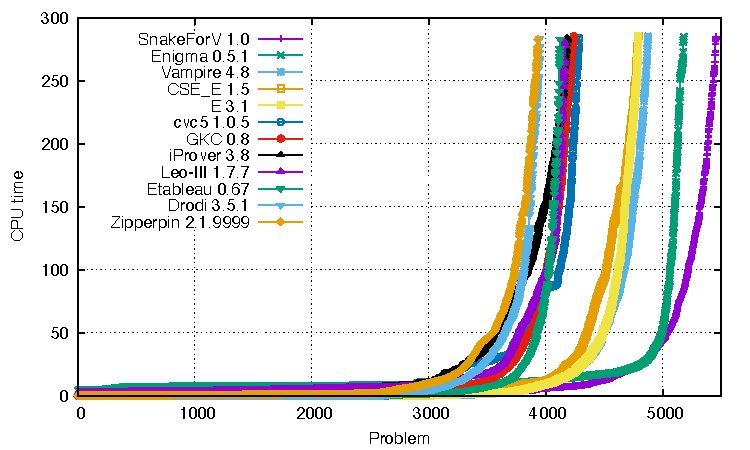
\includegraphics[width=0.6\textwidth]{Plots/FOF_THM_RFO_PPP/FOF_THM_RFO_PPP}
\vspace*{-1em}
\caption{CPU times for {\tt FOF\_THM\_RFO\_*}}
\label{PPPPlot}
\end{figure}

%--------------------------------------------------------------------------------------------------
\section{Analysis Processes}
\label{AnalysisProcesses}

%--------------------------------------------------------------------------------------------------
\subsection{Analysis Data}
\label{AnalysisData}

The analyses performed in this assessment use the TPTP problem ratings, and historical data about 
which ATP systems solved which problems in each TPTP release.
The data was extracted from the {\tt ProblemAndSolutionStatistics} file that accompanies each TPTP 
release, which summarizes information from the header fields of the TPTP problem files and
corresponding TSTP solution files.
As explained in Section~\ref{TSTP}, TSTP data starting from TPTP v6.3.0 in November 2015 has been
used, taking snapshots at each TPTP edition up to v8.2.0.

Before analysis the rating data was cleaned as follows:

\vspace*{-0.5em}
\paragraph{Cleaning for Bias:}
The TPTP tags problems that are designed specifically to be suited or ill-suited to some ATP 
system, calculus, or control strategy as {\em biased}. 
% This includes the {\tt SYN000} problems, which are designed for test ATP systems' parsers.
The biased problems were excluded from the analyses.

\vspace*{-0.5em}
\paragraph{Cleaning for Bugfixes:}
Over time some problems have had to be removed from the TPTP because they are renamed, duplicates, 
wrongly formulated, etc.
Such problems in a TPTP release are thus not in subsequent releases.
The removed problems were excluded from the analyses.

\vspace*{-0.5em}
\paragraph{Cleaning for the Past:}
Problems are added to the TPTP in each release, and corresponding TSTP data is generated using 
the available ATP systems.
As it is not possible to run all previously available ATP systems on new problems when they 
are added to the TPTP, it has been (quite reasonably) assumed that if a problem was unsolved by the 
current ATP systems when it was added to the TPTP (initial rating 1.00), then it would have been 
unsolved by previously available ATP systems.
The rating data was thus augmented for problems that were added after v6.3.0 and had an
initial rating of 1.00, by setting the problems' ratings in the prior TPTP releases to 1.00.
There were 1854 such problems.
This, however, can lead to an unfairly optimistic view of progress, because those retrospectively 
added 1.00 ratings increase the average problem rating in the past.
For problems that were solved when they were added to the TPTP (initial rating less than 1.00),
it is unknown if the previously available ATP systems would have been able to solve them.
Augmenting the rating data by setting the problems' ratings in prior TPTP releases to their 
initial rating of less than 1.00 could lead to a pessimistic view of progress, because those 
retrospectively added ratings decrease the average problem rating in the past.
In this work the rating data was augmented for problems that were added after v6.3.0 and 
had an initial rating less than 1.00, by setting the problems' ratings in the prior TPTP releases 
to their initial rating.
There were 2632 such problems.
The optimistic/pessimistic effect gets stronger when rating data is augmented for problems that
were added in more recent TPTP releases, and balance each other out in the analyses.

\vspace*{-0.5em}
\paragraph{Cleaning for Change:}
A counterintuitive feature of an individual problem's difficulty ratings is that they sometimes 
increase with time. 
It is counterintuitive because the problem has not changed.
(This was also noted in a prior analysis \cite{Sut17}.)
% where it was noted: ``The ratings generally 
% show a downward trend - there has been progress!'', but ``ratings can also increase when data 
% from new systems is added to the TSTP.''
Increases are caused by new ATP systems or system versions becoming available.
If a new system is not subsumed then its TSTP data is used in the rating process:
the ratings of problems that it solves decrease, but at the same time the ratings of problems that 
it does not solve increase -- you have to ``pay the piper''.\footnote{%
Conversely, if a system that was not subsumed becomes unavailable, it no longer contributes
TSTP data for new problems.
% The new problems have higher ratings than they would have had if the system had remained
% available.
% Since the TSTP data started being generated on StarExec this has been a rare occurrence, e.g.,
% Isabelle ran fine on StarExec Iowa, but did not port to StarExec Miami in 2018.
This phenomenon is rare (e.g., Isabelle ran fine on StarExec Iowa but did not port to StarExec 
Miami in 2018) and has not materially impacted the analyses of progress.} 
A common instance of this phenomenon is a new system that can solve some previously unsolved
(rating 1.00) problems, but that cannot solve a substantial number of problems that are solved
by other systems (rating less than 1.00).
In this work the anomaly is resolved by additionally looking at {\em monotonic ratings}:
if a problem's rating in a TPTP release is greater than it's previous rating, the monotonic 
rating is set to the previous lower rating.
Monotonized ratings make clear sense in the case of problems that were unsolved (rating 1.00) and 
were later solved by a new system (the rating drops to less than 1.00) -- if a problem is 
solved, it cannot become unsolved -- the solving system still exists in principle.
In cases where the rating is less than 1.00 monotonized ratings might be considered to be 
optimistic because ratings do have to ``pay the piper''.

%--------------------------------------------------------------------------------------------------
\subsection{Coherent SPC Sets}
\label{SPCSets}

Five of the analyses performed (see Section~\ref{AnalysisTypes}) require data from sets of 
problems with similar characteristics, so that the analysis results are wrt that type of problem.
The basis for such sets is the SPCs (see Section~\ref{SPCs}), which provide a fine-grained 
partitioning of the TPTP problems so that each SPC is coherent.
Some SPCs that capture compatible problem characteristics can be merged to form a 
{\em coherent SPC set}.

The coherent SPC sets used for the analyses are listed in Table~\ref{SPCSetsTable}.
The SPC set column lists the SPCs that are in the set, using the abbreviations given in 
Section~\ref{SPCs}.
Some noteworthy exclusions are:
typed extended first-order problems, because they were added to the TPTP only in v8.0.0;
typed polymorphic first-order and higher-order problems, because too few systems are 
capable of attempting the problems and generating the necessary TSTP data;
some SPCs that have too few problems, e.g., {\tt TF0\_CSA\_*\_NAR} and {\tt TF0\_SAT\_*\_NAR},
which combined have only 154 problems.

\begin{table*}[h!]
\renewcommand{\arraystretch}{1.5}
\center
\begin{tabular}{p{3.5cm}|p{8.0cm}}
\hline
SPC set & Description \\
\hline
{\tt CNF\_UNS\_RFO\_PEQ\_UEQ} &
Unsatisfiable really-first-order unit equality clauses. \\
{\tt CNF\_UNS\_RFO\_NEQ\_*}\enspace$\cup$ {\tt CNF\_UNS\_RFO\_SEQ\_*}\enspace$\cup$
{\tt CNF\_UNS\_RFO\_PEQ\_NUE} &
Unsatisfiable really first-order clauses that are not unit equality. \\
{\tt CNF\_SAT\_RFO\_*} &
Satisfiable really-first-order clauses. \\
{\tt FOF\_*\_PRP}\enspace$\cup$ {\tt FOF\_*\_EPR\_*}\enspace$\cup$
{\tt CNF\_*\_PRP}\enspace$\cup$ {\tt CNF\_*\_EPR\_*} &
Unsatisfiable and satisfiable propositional and effectively propositional clauses.
Un/Satisfiable is coherent because the problems are decidable. \\
{\tt FOF\_THM\_RFO\_*} &
Really first-order theorems, with or without equality. \\
{\tt FOF\_CSA\_RFO\_*}\enspace$\cup$ {\tt FOF\_SAT\_RFO\_*} &
Really first-order non-theorems and satisfiable sets, with and without equality. \\
{\tt TF0\_THM\_*\_NAR} &
Typed monomorphic first-order theorems, with and without equality, no arithmetic. \\
{\tt TF0\_THM\_*\_ARI} &
Typed monomorphic first-order theorems, with and without equality, with arithmetic. \\
{\tt TH0\_THM\_*\_NAR} &
Typed monomorphic higher-order theorems, with and without equality, no arithmetic. \\
\hline
\end{tabular}
\vspace*{0.5em}
\caption{Coherent SPC sets}
\label{SPCSetsTable}
\end{table*}

%--------------------------------------------------------------------------------------------------
\subsection{Six Analyses}
\label{AnalysisTypes}

The cleaned TPTP problems ratings and historical TSTP data has been used for six analyses of 
progress in ATP.
Individual problem ratings are used for the first analysis.
The other five analyses are wrt the coherent SPC sets described in Section~\ref{SPCSets}.

\vspace*{-0.5em}
\paragraph{First Solutions:}
Arguably the most successful use of ATP comes from the ``hammers'' \cite{BK+16} associated with 
Interactive Theorem Proving (ITP) systems, where the individual problems being solved are 
typically not of direct interest to the human users who are focussed on the larger task being 
addressed in the ITP system.
%  e.g., Sledgehammer \cite{PB10} for Isabelle \cite{NPW02}, 
% HOLyHammer \cite{KU14} for HOL Light \cite{Har09} and HOL4 \cite{SN08}, 
% MizAR \cite{KU15-M40} for Mizar \cite{GKN10}.
In contrast, the use of ATP by practitioners to solve individual problems that have resisted
manual approaches is less common and possibly less successful, but the sparsity makes successes 
particularly noteworthy. 
First solutions of problems that are of direct interest to humans are indications of progress.
Such problems are identifiable by (i)~the rating decreasing from 1.00, and (ii)~evidence that the 
problem is of direct interest to some humans.

\vspace*{-0.5em}
\paragraph{Average difficulty ratings:}
This is the average problem difficulty rating, and the average monotonized difficulty rating.
(This approach was used in \cite{SFS01}.)
% The ratings are updated in each TPTP release, so that as time goes by and ATP systems improve 
% the ratings decrease
As the problems are unchanged (they are not actually getting easier), decreases are 
evidence of progress in ATP systems.

\vspace*{-0.5em}
\paragraph{Never-solved:}
This is the fraction of problems that were unsolved (rating 1.00) in all TPTP releases 
up to each TPTP release, relative to the number in v6.3.0.
(The converse of this is plotted in \cite{SSP21}.)
Decreases are evidence of progress.
% with fewer problems being unsolved by some ATP system.
% This analysis uses the cleaned ratings data, averaged over the problems in each coherent SPC set.
% CS OBJECTS In order for this analysis to be meaningful 

\vspace*{-0.5em}
\paragraph{Solved:}
This is the fraction of problems solved less the least solved across all releases, 
relative to the most solved less the least solved across all releases.
The releases with a 1.00 value are those in which the most problems were solved, and those with
0.00 had the least number solved.
Increases are evidence of progress.
% with more problems being solved by the 
% state-of-the-art (See Section~\ref{Ratings}) in ATP systems.

\vspace*{-0.5em}
\paragraph{Always-easy:}
This is the converse of Never-solved -- the fraction of problems that were easy (rating 0.00) in 
all TPTP releases back to each TPTP release, relative to the number in v8.2.0.
Increases are evidence of progress.
% with more problems being solved by the 
% state-of-the-art (See Section~\ref{Ratings}) in ATP systems.

\vspace*{-0.5em}
\paragraph{Shapley value:}
% This measures the progress of systems through their marginal contributions and Shapley 
% values \cite{XH+12}.
A State-of-the-Art (SotA) ATP system for a TPTP release is defined as one that solves the union 
of the problems solved by the individual ATP systems, e.g., by using competition parallelism
\cite{SS94-PPAI}.
First, temporal Shapley analysis \cite{KF+19} is used to measure the SotA systems' contributions to 
progress, and peaks indicate strong progress.
Next, (non-temporal) Shapley analysis \cite{FK+16} is used to measure the contributions of the
individual systems in each release.
Finally, temporal Shapley analysis for all systems in all releases is used to measure the
contributions of the individual system versions when they were introduced.
% , which reveals the numbers of problems they solved but that had never been solved before.
The latter two analyses were used to provide insights for the commentary about the systems' 
performances (they are not plotted in Section~\ref{Evidence}).

%% \begin{enumerate}
%% \item Extract all data from TSTP, starting from v6.2.0, per above.
%% \item Fill right for problems added after v6.2.0 if their rating started at 1.00. 
%% %      If the rating started below 1.00, that assumes that earlier systems would have been
%% %      equally able to solve it, which might be kind to those systems.
%% %      The result is less apparent progress before then.
%% \item Fill left for missing data
%%       \begin{itemize}
%%       \item Do not allow a problem to become more difficult.
%%       \end{itemize}
%% \item Remove problems with missing ratings
%% \item Extract ratings for a chosen set of SPCs 
%% \item Compute summary data
%%       \begin{itemize}
%%       \item Number of problem rows
%%       \item Average rating
%%       \item Number of problem rows with rating 0.00 to 0.99
%%       \item Fraction of problem rows with rating 0.00 to 0.99
%%       \item Number of problem rows with rating 0.00
%%       \item Fraction of problem rows with rating 0.00
%%       \item Number of problem rows with rating 0.01 to 0.99
%%       \item Fraction of problem rows with rating 0.01 to 0.99
%%       \item Number of problem rows with rating 1.00
%%       \item Fraction of problem rows with rating 1.00
%%       \end{itemize}
%% \item Plot by date
%%       \begin{itemize}
%%       \item Fraction of problem rows with rating 0.00 to 0.99
%%       \item Average rating
%%       % \item Fraction of problem rows with rating 0.00
%%       % \item Fraction of problem rows with rating 0.01 to 0.99
%%       % \item Fraction of problem rows with rating 1.00
%%       \item Temporal Shapley value
%%       \end{itemize}
%% \end{enumerate}

%--------------------------------------------------------------------------------------------------
\section{Evidence of Progress}
\label{Evidence}

%--------------------------------------------------------------------------------------------------
\subsection{First Solutions}
\label{FirstSolutions}

There are some nice examples of ATP systems finding first solutions to problems that are
of direct interest to humans~\ldots

\begin{itemize}
\item Model finding ATP systems were used to solve previously open problems concerning the 
      existence of quasigroups satisfying certain additional conditions \cite{SFS95}.
      Many examples are in the {\tt GRP} domain of the TPTP.
\item The solution of the Robbins problem\footnote{%
      The Robbins problem was posed in personal communications between Edward Huntington,
      Herbert Robbins, and Alfred Tarski.
      The background is given in 
      \href{https://en.wikipedia.org/wiki/Robbins_algebra}{en.wikipedia.org/wiki/Robbins\_algebra}.}
      by the specialist ATP system EQP \cite{McC97} 
      in 1996 was a noteworthy success, as the problem had defied the efforts of eminent 
      mathematicians \cite{HMT71}.
      It is {\tt ROB001-1} in the TPTP, and still has a rating of 1.00 because 
      it has not been solved by a non-specialist ATP system.
\item The first inner five-segment theorem of Tarski's geometry \cite{SST83} was first 
      automatically proved by E \cite{Sch13-LPAR} in 2019, after being posed by Quaife in 
      1989 \cite{Qua89}.
      It is problem {\tt GEO033-2} in the TPTP.
\item The proof of the consistency of an encoding of a large fragment of a high school textbook
      on biology \cite{CDI13} by iProver \cite{Kor08} in 2021 showed how new techniques could
      be used to find models in large theories.
      It is problem {\tt BIO001+1} in the TPTP.
\item Larry Wos' challenge to find a ``circle of pure proofs'' that shows the equivalence
      of the four Moufang identities \cite{Wos19} was met by careful application \cite{Ver22} of
      Otter \cite{McC03-Otter} in 2021.
      While those specific problems are not in the TPTP, many related problems are in the
      ring theory ({\tt RNG}) domain of the TPTP.
\end{itemize}

%--------------------------------------------------------------------------------------------------
\subsection{Solutions and Ratings}
\label{SolutionsAndRatings}

A total of 25325 problems were analysed over the coherent SPCs, of which 19762 (78\%) were 
solved in TPTP v6.3.0, increasing to 20227 (80\%) in v8.2.0.
Of the 25325 problems, 5563 (22\%) were unsolved when they were added to the TPTP, of which 1009 
(4\%) were solved in some release by v8.2.0. 
Conversely, there were 8984 problems (35\%) that had a rating of 0.00 in v8.2.0, of which 2965 
(12\%) had a higher rating in some preceding release.
These overall figures provide evidence of overall progress, but the contributions vary across
the coherent SPC sets.
Figures~\ref{Plot_CNF_UEQ}-\ref{Plot_TH0_THM_NAR} plot the values for each coherent SPC set
for the latter five analyses described in Section~\ref{AnalysisTypes}.\footnote{%
Data: \href{https://github.com/GeoffsPapers/ATPProgress2024/raw/master/DataForAnalysis}{github.com/GeoffsPapers/ATPProgress2024/raw/master/DataForAnalysis}}
The captions provide the numbers of `P'roblems in TPTP v8.2.0, the number left for analysis 
after the data cleaning, and the numbers of `N'ever-solved, `S'olved, and `A'lways-easy problems 
in releases v6.3.0-v8.2.0.

Figures~\ref{Plot_CNF_UEQ} to \ref{Plot_FOF_CSA_SAT_RFO} plot the values for the CNF- and
FOF-based coherent SPC sets.
CNF is now the ``assembly language'' of most ATP systems, which typically translate more
expressive logics down to CNF.
As such, progress in CNF typically contributes to progress in other SPCs.

{\tt CNF\_UNS\_RFO\_PEQ\_UEQ} showed progress in v6.4.0 due to the strong performance of
Twee~2.0 \cite{Sma21}, which made a lot more problems always-easy by v7.0.0.
Also in v6.4.0, Waldmeister~710 \cite{LH02} solved five problems that had never been solved 
before.
In v7.4.0 E~2.5 made a strong contribution, then in v8.1.0 Twee~2.4 made another strong 
contribution, alongside CSE\_E~1.3 \cite{XL+18}.
Waldmeister~710 had the highest Shapley value across all the releases, but in
v8.1.0 both Twee and CSE\_E solved more problems than Waldmeister.
The lowest number of problems solved was in v7.5.0 and v8.0.0, when 23 fewer problems were solved
than in v7.4.0 -- not many in the context of the 1034 solved in v7.4.0.
The only discernible common feature of those 23 problems is that they had ratings over 0.90 in 
v7.4.0.
Apparently some changes in the ATP system versions from v7.4.0 to v7.5.0 made the problems
unsolvable in v7.5.0, and further changes reversed the situation for v8.1.0 when 1043 problems
were solved.
% {\tt CNF\_UNS\_RFO\_PEQ\_UEQ} is interesting because it is possible to use complete search 
% strategies, so that in a strategy schedule the individual strategies can be run for longer 
% periods with hope of solving harder problems \cite{SD24-CASC}.
 
{\tt CNF\_UNS\_RFO\_*\_NUE} had a small but quite consistent decline in the problem ratings, 
indicating some progress.
The big advances were in v7.0.0 when Vampire~4.2 performed well, including solving 33 problems
that had never been solved before.
In v8.2.0 SnakeForV~1.0 solved 26 problems that had never been solved before.
% The numbers of always-easy and never-solved problems improved correspondingly.
The biggest drop in problems solved was between v7.2.0 and v7.3.0, when 66 fewer problems were
solved.
The largest increase in problems solved was between v8.1.0 and v8.2.0, when 50 more problems
were solved.
SnakeForV was again the big contributor to the increase.
SnakeForV is interesting, as it is a variant of Vampire with a different approach to the strategy
scheduling \cite{Sud22}.

{\tt CNF\_SAT\_RFO\_*} had only one high point, in v6.4.0 when Vampire~4.0.5 made a strong
contribution, including solving four problems that had never been solved before.
The sudden drop in problems solved in v7.0.0 was due to Prover9~1105 \cite{McC-Prover9-URL}
data not being available; the reason is lost in the mists of time, but it is interesting to note 
that the older system was able to solve some problems that other systems could not.
By v7.1.0 new systems had taken up the slack.
The plots are all quite stable from v7.1.0 onwards.

{\tt \{FOF,CNF\}\_*\_EPR\_*} had two points of progress, the first in v7.0.0 and the second in
v7.3.0.
In v7.0.0 the progress came from iProver~2.6 that had integrated an abstraction-refinement 
framework \cite{HK17}, and Vampire~4.2 that had some changes in its model building.
Between them they solved five problems that had never been solved before.
In v7.3.0 iProver~3.0 integrated superposition \cite{DK20}.
The number of problems solved increased continuously until v8.2.0. 
The drop in v8.2.0 
% was only 17 fewer problems solved than in v8.1.0, and 
was due to poorer performances by the new iProver~3.7, SnakeForV~1.0, and Vampire~4.7.
These systems share the same FOF to CNF translator, which might have been the source of the
common change.

{\tt FOF\_THM\_RFO\_*} is the best known of the FOF-based SPCs, with the most ATP systems able 
to attempt the problems, and is the target of most new systems.
The problem difficulty ratings are quite flat, but the number of problems solved increased quite 
regularly, from 6086 in v6.3.0 to 6235 in v8.2.0.
The largest step of progress came in v7.0.0 when Vampire~4.2 solved 72 problems that had never 
been solved before, thanks to improvements in preprocessing.
ET~0.2 \cite{KS+15} also contributed to the progress in v7.0.0.
In v7.4.0 Enigma~0.4 \cite{JU17,JC+20} was a new system that made a strong contribution to 
progress.
Vampire~4.5 also contributed to progress in v7.4.0, with a new layered clause selection approach 
\cite{GS20} and a new subsumption demodulation rule \cite{GKR20}.

{\tt FOF\_\{CSA,SAT\}\_RFO\_*} is also well known, and along with its typed first-order
counterpart (not analysed due to insufficient data) is important for applications, 
e.g.,~\cite{DKW08}.
The largest sign of progress was in v6.4.0.
The main contributors were Vampire~4.0.5 with improvements to its satisfiability checking,
and iProver~2.5 with restructured core data structures and improved preprocessing including 
predicated elimination.
Vampire~4.0.5 solved 10 problems that had never been solved before.
There is a drop of 10 problems solved from v8.0.0 to v8.2.0.
As in {\tt CNF\_UNS\_RFO\_PEQ\_UEQ}, there is no discernible common feature of those 10 problems,
and their ratings were at most 0.75.
This again shows that the set of problems solved by evolving versions of systems does not grow
monotonically.

\begin{figure}[b!]
\centering
\begin{minipage}[t]{.49\textwidth}
  \centering
  \includegraphics[width=\textwidth]{Plots/GNUPlots/CNF_UNS_RFO_UEQ.pdf}
  \vspace*{-2em}
  \caption{{\tt CNF\_UNS\_RFO\_PEQ\_UEQ} \\ 
           {\scriptsize P:1140-1140 N:120-86 S:1020-1049 A:38-233}}
  \label{Plot_CNF_UEQ}
\end{minipage}
\begin{minipage}[t]{.49\textwidth}
  \centering
  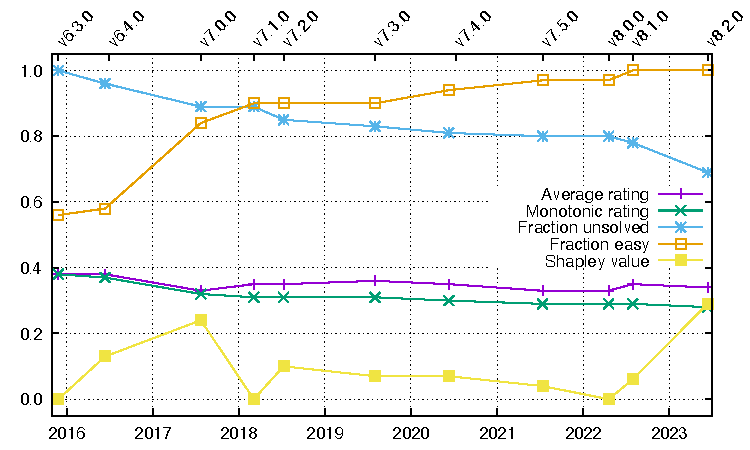
\includegraphics[width=\textwidth]{Plots/GNUPlots/CNF_UNS_RFO_NUE.pdf}
  \vspace*{-2em}
  \caption{{\tt CNF\_UNS\_RFO\_*\_NUE} \\
           {\scriptsize P:4445-4441 N:569-391 S:3873-3966 A:1004-1780}}
  \label{Plot_CNF_UNS}
\end{minipage}
\begin{minipage}[t]{.49\textwidth}
  \centering
  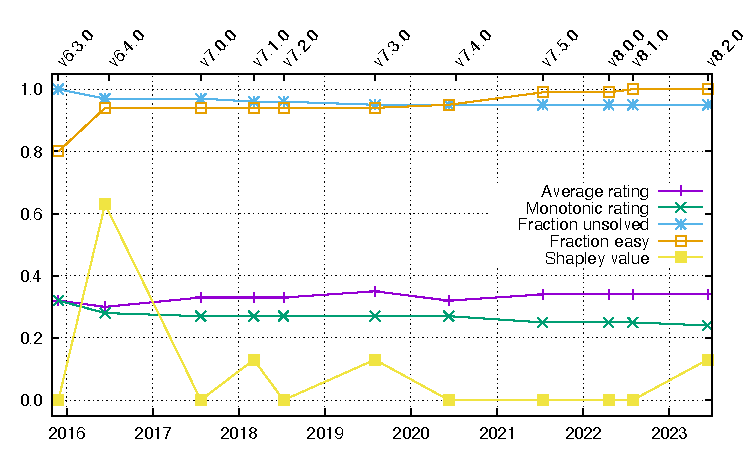
\includegraphics[width=\textwidth]{Plots/GNUPlots/CNF_SAT_RFO.pdf}
  \vspace*{-2em}
  \caption{{\tt CNF\_SAT\_RFO\_*} \\
           {\scriptsize P:1044-1042 N:155-147 S:887-889 A:476-598}}
  \label{Plot_CNF_SAT}
\end{minipage}
\begin{minipage}[t]{.49\textwidth}
  \centering
  \includegraphics[width=\textwidth]{Plots/GNUPlots/FOF_CNF_EPR.pdf}
  \vspace*{-2em}
  \caption{{\tt \{FOF,CNF\}\_*\_EPR\_*} \\
           {\scriptsize P:1457-1425 N:78-43 S:1347-1360 A:1027-1311}}
  \label{Plot_FOF_CNF_EPR}
\end{minipage}
\begin{minipage}[t]{.49\textwidth}
  \centering
  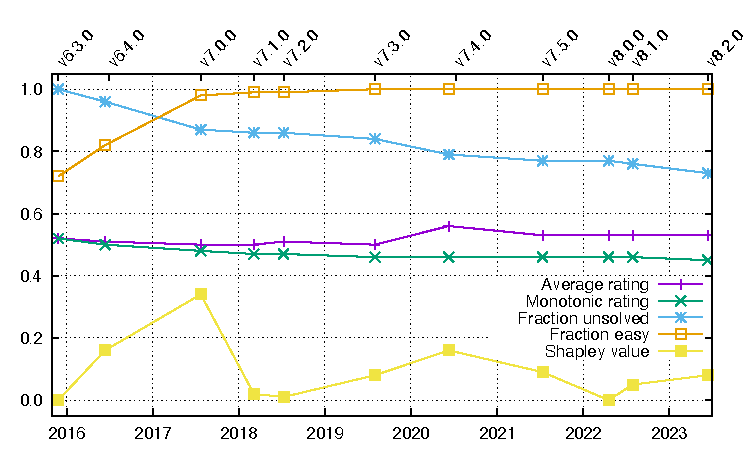
\includegraphics[width=\textwidth]{Plots/GNUPlots/FOF_THM_RFO.pdf}
  \vspace*{-2em}
  \caption{{\tt FOF\_THM\_RFO\_*} \\
           {\scriptsize P:7204-7202 N:1116-818 S:6086-6235 A:696-971}}
  \label{Plot_FOF_THM_RFO}
\end{minipage}
\begin{minipage}[t]{.49\textwidth}
  \centering
  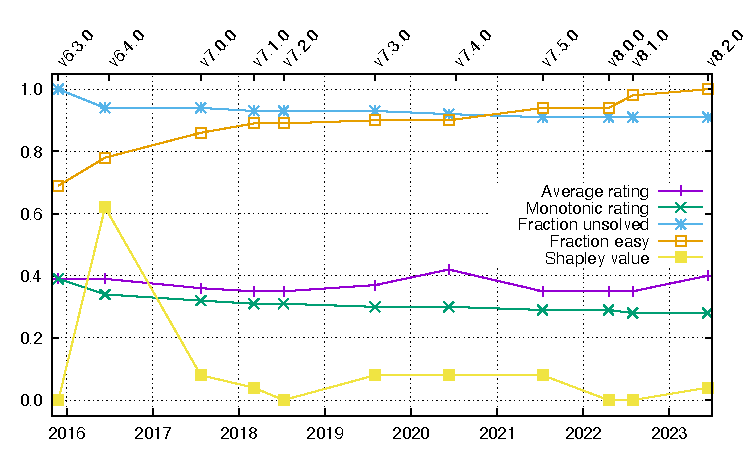
\includegraphics[width=\textwidth]{Plots/GNUPlots/FOF_CSA_SAT_RFO.pdf}
  \vspace*{-2em}
  \caption{{\tt FOF\_\{CSA,SAT\}\_RFO\_*} \\
           {\scriptsize P:1329-1028 N:282-256 S:746-753 A:481-709}}
  \label{Plot_FOF_CSA_SAT_RFO}
\end{minipage}
\end{figure}

Figures~\ref{Plot_TF0_THM_NAR} to \ref{Plot_TH0_THM_NAR} plot the values for the TFF- and
THF-based coherent SPC sets.
{\tt TF0\_THM\_*\_NAR} uses the simplest of the typed TPTP languages.
In v7.0.0 there was progress thanks to Vampire~4.2 and CVC4~1.5.2 \cite{BC+11}.
In v8.2.0 there was progress thanks to SnakeForV~1.0.
In between those points of progress there was a drop in the number of problems solved, from
282 in v7.4.0 down to 260 in v7.5.0, apparently due to poorer performance of CVC4~1.9
in v7.5.0 compared to that of CVC4~1.7 in v7.4.0.

{\tt TF0\_THM\_*\_ARI} is important because it uses the simplest TPTP language that 
includes arithmetic, which occurs naturally in application areas \cite{KK+23,BF+15,PB10}.
There was clearly some significant progress in v6.4.0 as many problems were solved for the
first time by Vampire~4.0.5, which had integrated Z3 \cite{dMB08} since Vampire~4.0.
This contributed to the increase in the number of problems solved, from 915 in v6.3.0 to 1009 
in v6.4.0.
CVC4~1.5 \cite{BC+11} and Princess~150706 \cite{Rue08} also performed well.

{\tt TH0\_THM\_*\_NAR} uses typed higher-order logic, and despite using a more expressive
language than the {\tt TF0\_*} SPCs, has been the focus of ATP system development longer 
\cite{SB10,SS+12}.
The problem ratings declined moderately, and there were bursts of progress in v7.0.0 and v7.5.0.
The progress in v7.0.0 was largely thanks to Satallax~3.2 \cite{Bro12}, which included a SInE-like 
\cite{HV11} procedure for premise selection that enabled it to solve some large problems that 
were previously out of reach. 
That progress increased the number of always-easy problems by v7.1.0.
In v7.5.0 Zipperposition~2.0 \cite{BB+19-CADE} improved over the previous version, and solved
18 problems that had never been solved before.
% that had dominated the SPC since 2013.
% Despite Vampire's improving performance on {\tt THF\_*} problems (noted above), it took until
% Vampire~4.8 in 2023 to surpass Zipperposition, and that performance data was collected after v8.2.0.

Figure~\ref{Ratings_v5.0.0_v6.4.0} was presented (verbatim) in a prior analysis done at TPTP 
release v6.4.0 \cite{Sut17}.
The figure plotted the average ratings for the 14527 problems that have been unchanged in the 
TPTP since v5.0.0, and whose ratings had not been stuck at 0.00 or 1.00 since v5.0.0. 
It was noted in \cite{Sut17}: 
``The ratings generally show a downward trend - there has been progress!''.
The same analysis has now been done at TPTP release v8.2.0, for the 16236 problems that have been 
unchanged in the TPTP since v6.3.0, and whose ratings have not been stuck at 0.00 or 1.00 since 
v6.3.0.
The two figures' plots dovetail quite well, which gives confidence that they really are comparable
(there are some minor differences caused by the data cleaning done for this work, and recent 
refinements to the rating calculations \cite{SD23-CASC,SD24-CASC}).
The older plots show a quite clear downward trend both overall and for the four types of problems,
while the new plots do not.
Possible reasons are discussed in the conclusion (Section~\ref{Conclusion}).

\begin{figure}[t!]
\centering
% \begin{figure}[h!]
% \centering
\begin{minipage}[t]{.49\textwidth}
  \centering
  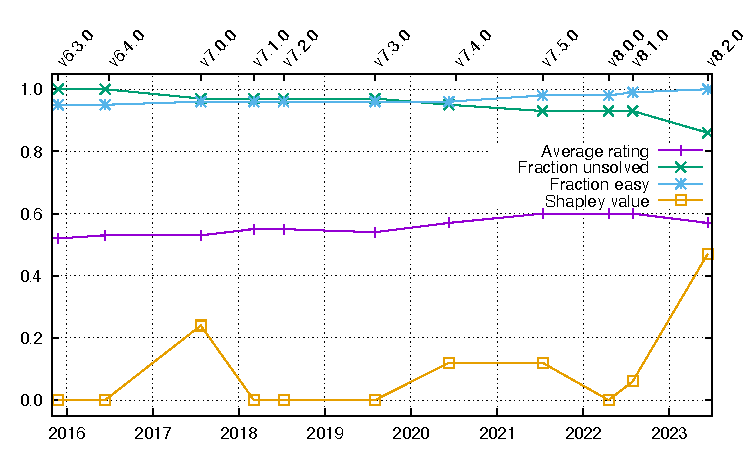
\includegraphics[width=\textwidth]{Plots/GNUPlots/TF0_THM_NAR.pdf}
  \vspace*{-2em}
  \caption{{\tt TF0\_THM\_*\_NAR} \\
           {\scriptsize P:400-397 N:120-103 S:277-268 A:117-123}}
  \label{Plot_TF0_THM_NAR}
\end{minipage}
\begin{minipage}[t]{.49\textwidth}
  \centering
  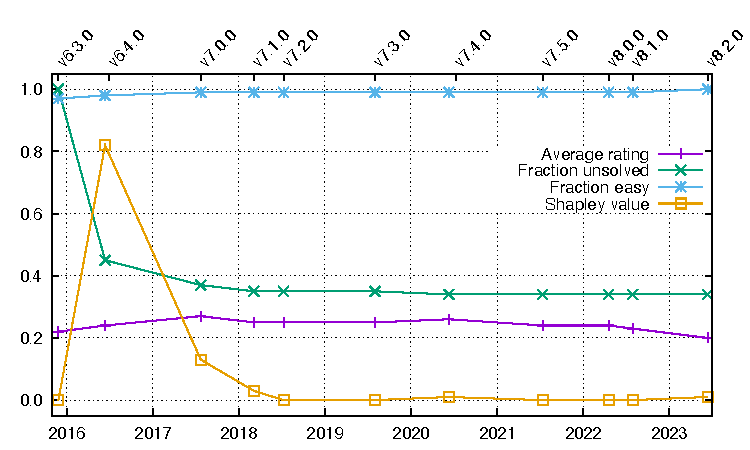
\includegraphics[width=\textwidth]{Plots/GNUPlots/TF0_THM_ARI.pdf}
  \vspace*{-2em}
  \caption{{\tt TF0\_THM\_*\_ARI} \\
           {\scriptsize P:1176-1087 N:172-58 S:915-1022 A:763-785}}
  \label{Plot_TF0_THM_ARI}
\end{minipage}
\begin{minipage}[t]{.49\textwidth}
  \centering
  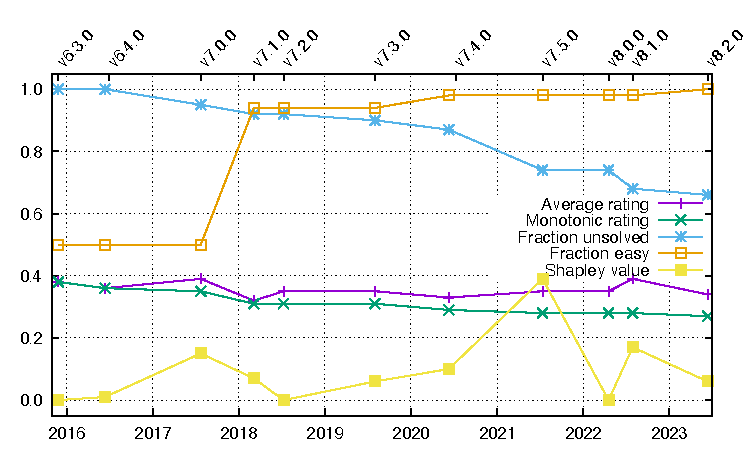
\includegraphics[width=\textwidth]{Plots/GNUPlots/TH0_THM_NAR.pdf}
  \vspace*{-2em}
  \caption{{\tt TH0\_THM\_*\_NAR} \\
           {\scriptsize PA:3189-3183 N:461-305 S:2722-2814 A:617-1244}}
  \label{Plot_TH0_THM_NAR}
\end{minipage}
\\
\begin{minipage}[t]{.49\textwidth}
  \centering
  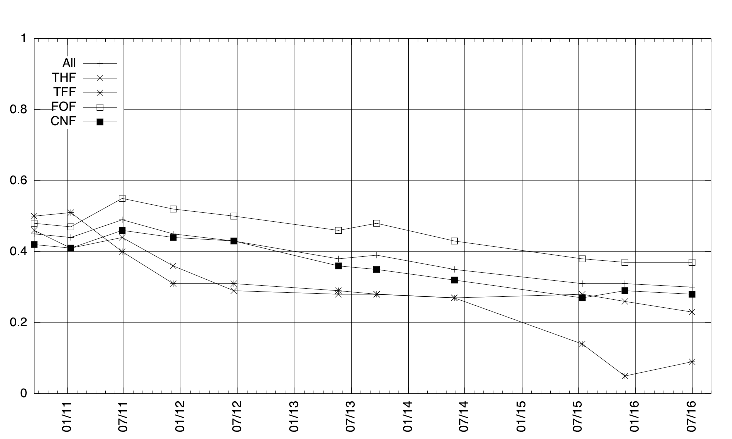
\includegraphics[width=\textwidth]{Plots/RatingsDecline_v5.0.0_v6.4.0.pdf}
  \vspace*{-2em}
  \caption{Ratings from v5.0.0 to v6.4.0}
  \label{Ratings_v5.0.0_v6.4.0}
\end{minipage}
\begin{minipage}[t]{.49\textwidth}
  \centering
  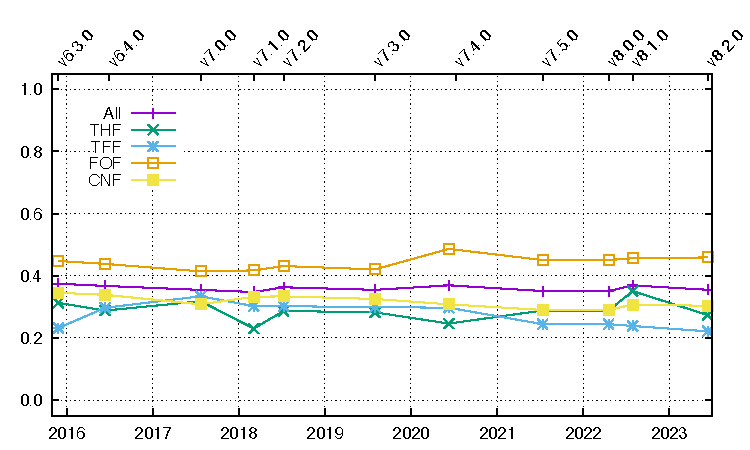
\includegraphics[width=\textwidth]{Plots/RatingsDecline_v6.3.0_v8.2.0.pdf}
  \vspace*{-2em}
  \caption{Ratings from v6.3.0 to v8.2.0}
  \label{Ratings_v6.3.0_v8.2.0}
\end{minipage}
\end{figure}

%--------------------------------------------------------------------------------------------------
\section{Conclusion}
\label{Conclusion}

This paper has presented an empirical assessment of progress in ATP, using data from the TPTP
World in TPTP v6.3.0 in 2015 to v8.2.0 in 2023.
The assessment has been in terms of six measures, divided into nine coherent SPC sets of problems
that are reasonably homogeneous for ATP systems.
The assessment shows that there has been progress in the last eight years, with stronger progress 
from v6.3.0 (2015) up to v7.1.0 (2018), but then a period of quiet until some more signs of 
progress in v8.2.0 (2023).
There have been some first solutions of problems that are of direct interest to humans,
a quite large number of first ATP solutions of problems from the TPTP, and
some noteworthy improvements in individual ATP systems.
The coherent SPCs with the strongest signs of progress were {\tt CNF\_UNS\_RFO\_PEQ\_UEQ} and
{\tt TH0\_THM\_*\_NAR}.

In terms of problem difficulty ratings, the monotonized ratings necessarily went down but the 
trend was not dramatic, and the raw ratings were generally stable.
This is in contrast to the clearly decreasing ratings from 2011 to 2016.
The reasons for that apparent slowing of progress are not definitely known, but we have thought of 
the following possible reasons:
\begin{itemize}
\item System developers have expended effort adding breadth of capability at the expense of 
      depth, e.g., 
      E -- processed only CNF and FOF up to 2015, added TF0 in 2017 \cite{SCV19}, TX0 and TH0 
           in 2019 \cite{VB+19};
      iProver -- processed only CNF and FOF up to 2015, added TF0 with arithmetic in 2021 
           (unpublished);
      Vampire -- processed only CNF, FOF, and TF0 up to 2015, added TX0 in 2016 \cite{KK+16}, 
           TF1 and TX1 in 2020 \cite{BR20-IJCAR}, and THF in several incarnations from 2019 to 
           2023 \cite{BR19,Bha20-Thesis,BRS23}.
\item The entry barrier to building new high-performance ATP systems is high, because top systems
      dominate the field and attract the best developer talent.
      In Maria Paola Bonacina's welcoming address at the Dagstuhl Seminar ``The Next Generation 
      of Deduction Systems: from Composition to Compositionality''\footnote{%
      \href{https://www.dagstuhl.de/23471}{www.dagstuhl.de/23471}} she referred to this as a
     ``crisis of growth''.
      % , as it becomes harder to make new systems, and instead features are 
      % incrementally added to existing systems.
      % In Pascal Fontaine's presentation ``On the Need for a Modular Approach for Automated 
      % Reasoners'' he referred to this as an ``Automated reasoning software crisis''.
\item New systems that take new approaches solve different subsets of SPCs have an impact on 
      problem difficulty ratings.
      For examples:
      CSE\_E \cite{XL+18} was new in 2018, combining the S-CS calculus with E;
      Zipperposition \cite{BB+21} was new in 2019, extending superposition to higher-order logic;
      Twee \cite{Sma21} was new in 2018, solving CNF and FOF problems by transformation to UEQ.
\item Time spent on machine learning based techniques, for axiom selection, e.g., 
      \cite{Urb06,KB14}, given clause selection, e.g., \cite{JU17-CICM,CA+21,AA+22-ML,MS23}), 
      learning for large problem corpora, e.g., \cite{KM+14,JU19,BL+19-ICML}, 
      and use of large language models to improve ATP performance \cite{WX+23,AS+23},
      is focussed largely on sets of many quite similar problems over one fixed signature.
      The progress made in that usage does not contribute directly to general progress in
      solving individual problems with different signatures, as measured in this work.
\item SMT solvers have been in existence since the late 1970s \cite{NO79}, blossomed fully
      in the early 2000s, and has attracted ever-increasing interest since then.
      Some ATP systems have been adapted to solving SMT problems, e.g., Vampire has been entered
      into SMT-COMP since 2016, and iProver since 2021.
      This is all good work, but has possibly diverted developer energy from ATP to SMT.
\item In \cite{SD24-CASC} it was noted that CASC might be causing incremental development of ATP
      systems.
      This concern has been expressed as far back as CASC-JC in 2001 \cite{PSS02}.
      In response to this concern CASC-J12 will have a new ICU (I Challenge yoU) division that
      focusses on solving hard problems rather than solving more problems, hoping to stimulate
      new developments and progress.
\end{itemize}

This assessment of progress is based on ATP systems' abilities to solve problems.
Evaluation of other performance measures would be interesting, and some have been done
in other evaluations of logic-based systems.
These include measures such as resource usage and verifiability of proofs/models.
Evaluation of non-performance measures is often ignored, but for users might be just as
necessary.
These include measures such as 
the range of logics covered, 
ease of building and deploying,
portability to different hardware and operating system environments, 
availability of source code, 
quality of source code and its documentation,
licensing that permits a required level of use or modification, 
availability of user documentation, 
and (maybe most importantly!)
developer support.
These are topics for future assessments.

%--------------------------------------------------------------------------------------------------
\bibliographystyle{splncs04}
\bibliography{Bibliography}
%--------------------------------------------------------------------------------------------------
\end{document}
